\chapter{Systems Development}

\section{Introduction}
Creating good software requires good coding skills, so you can get the computer to do what you want. Additionally, however, it requires good "systems development" skills so that (1) your code is organized / quickly updateable by yourself and others and (2) designing the product your users want, rather than what you \emph{think} they want. Systems development is a useful concept not just for computer science projects, but for any type of product development. 

For code organization, we use \textbf{Application Programming Interfaces} (APIs), which are a set of functions and procedures to allow different portions of code in a big project to communicate with each other. For user-guided product design, we use \textbf{iterative design}, which is the process of making many imperfect iterations of a project to prototype to users before trying to make the final product. 

\section{Code Organization}

 \subsection{Modularity}
 \begin{definition}
 \textbf{Modularity} means that code can be separated into many smaller components that are relatively independent. 
 \end{definition}
 
Modularity has two primary benefits:
\begin{itemize}
\item \textbf{Teamwork}: It allows different people to work on different portions of the code without interfering with one another. This is how software companies like Google, Amazon, and Microsoft can have tens of thousands of teammembers all working on the same project.
\item \textbf{Updateability}: It ensures that if one portion of the code needs to be updated or fixed, the rest of the code will not be impacted. 
\end{itemize} 

To illustrate this, we will consider modularity's usefulness in cars. Cars are incredibly complicated, but they can be understood by considering them as a collection of interacting components. Each component has its own functionality and relationship to the rest of the car.  

A few components of a car include:
\begin{itemize}
\item Tires: a round object that can attach to an axle
\item Engine: a device that can spin an axle
\item Axle: a rod that can be connected in the center to an engine, and at the edges to tires
\end{itemize} 

\begin{figure}
	\centering
	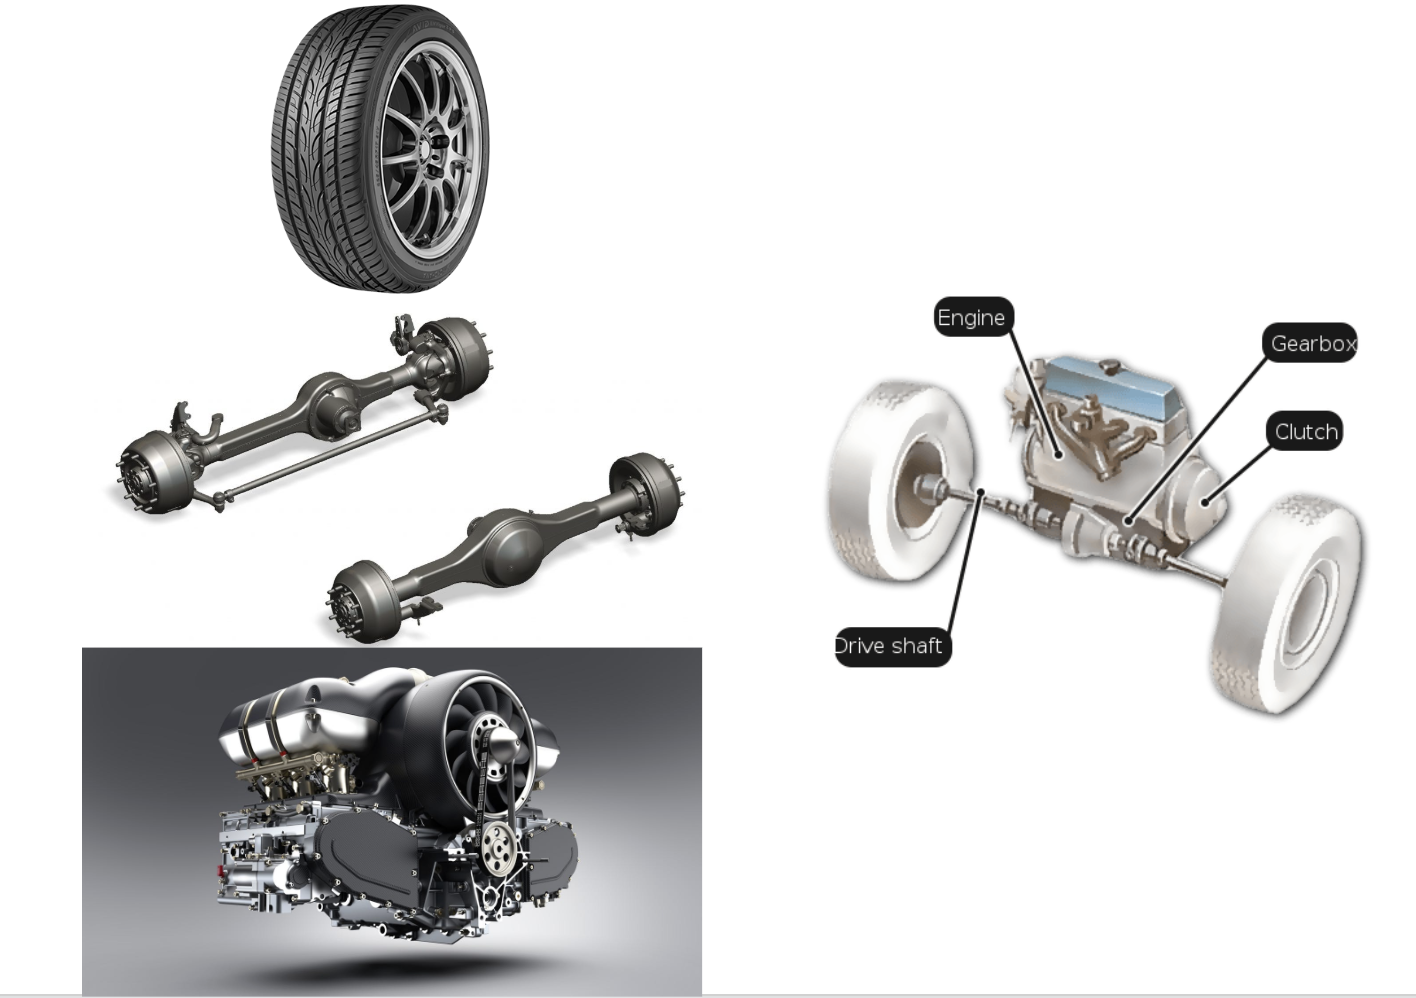
\includegraphics[width=0.5\textwidth]{images/car_example}
	\caption{Tires, engine, and axle can be combined to make the core axle-tire-engine unit of a car.}
\end{figure}

There are different ways to design each of these. They can each be made from a number of materials, and there are different sizes and varieties of each (e.g. 4 vs 6 cylinder engine, snow vs all-season tires, etc.). Furthermore, any \textit{combination} of these different varieties can be put together: we can change the type of tires we have without thinking about what type of axle or motor is in the car. 

\begin{figure}
	\centering
	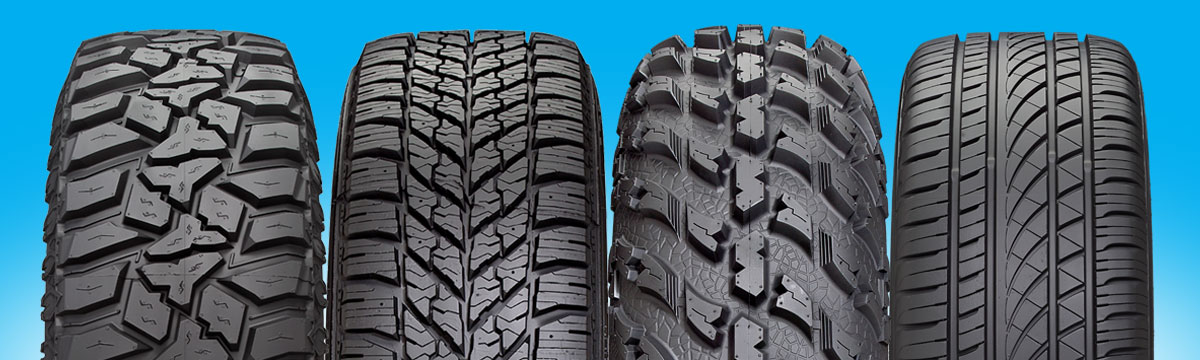
\includegraphics[width=0.5\textwidth]{images/tires.jpg}
	\caption{A variety of tires are available, and each must simply (1) be built to roll and (2) be connectable to an axle}
\end{figure}

We will now look at the benefits of this modularity in car design:

\begin{itemize}
	\item \textbf{Teamwork}: Car companies can divide up labor in multiple teams, and those teams won't interfere with each other as they work. One team can spend months developing the axle: finding the right alloy, shape, and weight to handle the load from the car. Another team can spend months developing the engine: trying out different arrangements of the cylinders or different numbers of cylinders. What's more, car manufacturers almost always outsource the production of their tires to tire manufacturers: they leave the decisions on the type of rubber and treads to a team totally outside of their company. The modularity of the car allows these teams to work totally separately, with the only communication between them the above list: the tire must roll and attach to an axle; the engine must spin the axle; and the axle must connect to the engine and the tires. Once the teams agree on the way they will bolt the systems together, they no longer have to communicate. 
    
	\item \textbf{Updateability}: Modularity allows car enthusiasts to upgrade and customize their vehicles without having to redesign the whole thing. If a vehicle owner wants to replace their V6 with a V8, they can do that as long as the connections between the motor and the rest of the vehicle are the same (i.e. the connection to the axle, to the fuel source, etc). If a vehicle owner wants to replace their all season tires for snow tires in the winter, they can do that as long as the connection with the rest of the vehicle is the same (i.e. the connection to the axle is the same). 
\end{itemize}

\begin{example}
Consider a small project team in a large company with two people: Alice and Bob. They are creating a food ordering system to replace waiters at a restaurant, which will present resturant-goers with a menu and allow them to directly place their order by clicking on their food choice. What are the components of such a system? How might Alice and Bob divide up the labor? 
\end{example}

As with many systems and apps, we can consider this system to have 2 primary components: a \textbf{frontend}, and a \textbf{backend}. The frontend is what the customer interacts with (the buttons and graphics). The backend is the behind-the-scenes computation and processing necessary so that the frontend functions as the user expects (e.g. transmitting information to be presented to users or doing mathematical calculations). In our example of writing a food delivery system, this might look like:
\begin{itemize}
	\item \textbf{Frontend}: Presents a scrollable list of menu options to the user. Allows users to click on any option, and sends that info to the backend. 
	\item \textbf{Backend}: Takes in a food choice from the frontend, and generates and sends a notification to the chef in the kitchen to "start preparing the choice." 
\end{itemize}

In our example, Bob might work on the frontend: making a beautiful menu with pictures of food, good descriptions, and a nice "order" button. 

Alice might work on the backend: ensuring that whatever food choice is chosen gets reliably transmitted to the kitchen and presented to the chef. 

\subsection{APIs}
\begin{definition}
An \textbf{Application Programming Interface}, or API, is a contract between components in a system, expressing what each component can expect from the others. 
\end{definition}

Building on the previous section's example of a vehicle, we can consider the API between the engine manufacturer and the vehicle manufacturer. 

The engine manufacturer can expect the vehicle to
\begin{itemize}
	\item have an axle 
	\item have a fuel source
	\item have a cooling source
	\item have a control system
\end{itemize}

The vehicle manufacturer the engine to
\begin{itemize}
	\item attach to an axle
	\item spin at a given revolution speed
\end{itemize}

As we saw in the previous section, this type of contract allows division of labor between different teams working on a project to ensure that they can work independently: as the engine manufacturer, 

Another API exists between a driver and the manufacturer: the driver can expect the car to have a 
\begin{itemize}
	\item device to turn on/off the car
	\item device to steer the car
	\item device to accelerate the car
	\item  device to decelerate the car
\end{itemize}

The car maker can expect the driver to have
\begin{itemize}
	\item arms and hands that can turn and push 
	\item feet and legs that can press 
\end{itemize}

\begin{example}
Make the API between an ATM and a user. 
\end{example}

From the perspective of a user, an ATM's purpose is to take in a credit car and a specified dollar amount from a user, and output the requested amount of money. The user can expect an ATM to
\begin{itemize}
	\item read their credit card
	\item specify the card's PIN number
	\item specify a requested dollar amount
	\item output money and notify their bank of the transaction
\end{itemize}

An ATM can expect the user to
\begin{itemize}
	\item have a credit card
	\item type with their fingers
	\item read and respond to prompts on the screen
\end{itemize}

Note that a problem with the API translates to a problem with the end-product. This API doesn't guarantee that a blind person will be able to use the ATM, for example (they won't be able to read). 

\begin{example}
Make the API between an ATM and a bank.
\end{example}

From the perspective of a bank, an ATM's purpose is to send in credit card info and the requested dollar amount, and fulfill a user request for money only if the bank authenticates the request. 

The bank can expect an ATM to
\begin{itemize}
	\item accurately send the bank credit card info and a PIN
	\item accurately send the bank the requested dollar amount
	\item complete the user's transaction only if the bank sends back a confirmation
\end{itemize}

The ATM can expect the bank to
\begin{itemize}
	\item receive credit card info and a PIN
	\item send back a confirmation or denial 
\end{itemize}

\section{User-oriented Design}

\subsection{Waterfall vs Iterative Design}

\begin{example}
Using 
\begin{itemize}
	\item 10 sticks of dry spaghetti
	\item one foot of string
	\item one foot of tape
\end{itemize}

build the highest tower possible in 6 minutes.

Adapted from https://tinkerlab.com/spaghetti-tower-marshmallow-challenge/
\end{example}

This activity generally demonstrates that iteration trumps pre-planning. It's faster to just trying out imperfect designs than to try to wait for a perfect idea. With a 6 minute time limit, iteration tends to work out better than pre-planning. 

\begin{definition}
\textbf{Waterfall design} is a development process in which each stage of development is finished before the next is started. 
\end{definition}

The components of waterfall design, adapted from https://airbrake.io/blog/sdlc/waterfall-model, are the following:
\begin{enumerate}
	\item Requirements: define what the application should do (essentially, write the API between a user and your product)
	\item Design: decide what the product will look like based on the requirements, and how it will be implemented
	\item Implementation: build the product based on the design
	\item Deployment: release the product to the users
\end{enumerate}

\begin{figure}
	\centering
	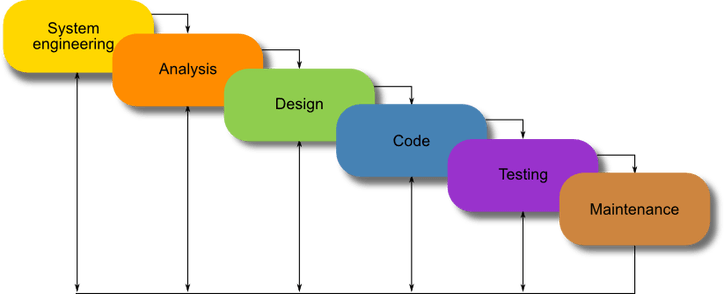
\includegraphics[width=0.5\textwidth]{images/waterfall.png}
	\caption{Waterfall design, courtesy https://airbrake.io/blog/sdlc/waterfall-model}
\end{figure}

In waterfall design, mistakes early in the process can kill you. You might spend a lot of time and money going through the full waterfall and developing a final product and then realize that the requirements were wrong. Going back to a previous example, suppose you had designed an ATM thinking that users would be able to read and later found out that blind users must also be able to access the ATM. You would have to completely redesign the system, perhaps having to put speakers into the ATM so that the prompts can be read aloud to the user. 

\begin{definition}
In \textbf{iterative design}, many iterations of a project are built and floated to users with the expectation that the requirements and design may need to be adjusted in further iterations. 
\end{definition}

Iterative design entails going through the same 4 steps of specifying requirements, drafting a design, implementing, then deploying. However, less time and money is invested into trying to make the first iteration perfect. The first iteration of a project might look horrible, but users will be able to tell you the fundamental flaws (such as missing requirements) before you start implementing a perfect product for the wrong problem. 

Iterative design is also used in drawing. As shown in \autoref{fig:owl}, professional artists start with a rough sketch of an object before starting to fill in details. The first iteration (top) doesn't look very good, but you might find out that you're missing basic requirements: you might be missing certain body parts, or decide you'd like to add a background or another object. By the second iteration, things look a little better, but you still might find more fundamental errors along the way. By the time you're ready to fill in all of the details in the bottom step, you're confident you're drawing the figure you want to draw. 

\begin{figure}
	\centering
	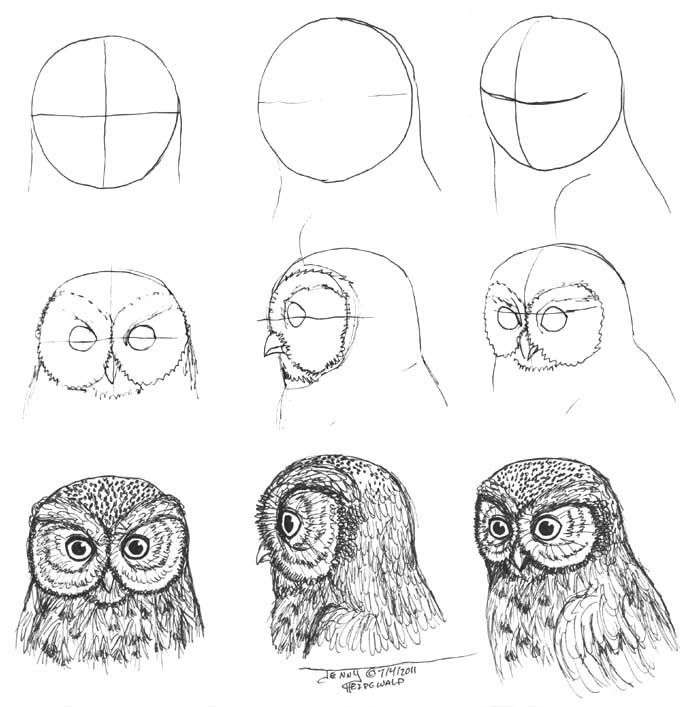
\includegraphics[width=0.5\textwidth]{images/owl.jpg}
	\caption{Iterative drawing of an owl. https://www.pinterest.com/pin/469289223655955022/}
	\label{fig:owl}
\end{figure}